\chapter{A Primer on Clustering in the SBM}

In this chapter we will introduce the Stochastic Blockmodel, as well as discuss the challenges in performing clustering on it. This will set the stage for discussing the experiments we performed with our Graph Neural Network to compare its clustering performance against the algorithmic benchmarks available for clustering on the Stochastic Blockmodel literature. 


The two challenges before us in studying clustering procedures rigorously are: 
\begin{center}
What is the ground truth?\\

What are the algorithmic guarantees?
\end{center}
Approached from a theoretical point of view, progress on these questions comes from studying special cases, oftentimes derived from generative probability models that capture much of the empirical behaviour.  One extremely well studied model is the Stochastic Blockmodel (one quick Google scholar search reveals about 8000 papers written on this topic, around 3000 of which since 2014).  It's a particularly simple and natural extension of the Erd\H{o}s Renyi random graph model, which exhibits community structure.  The randomness involved in the construction of the graph allows one to prove properties of the graph that hold asymptotically.  Despite the simplicity of its definition (given below), the SBM has proved fertile ground for testing algorithmic performance.  Additionally, theoretical guarantees for community detection in different families of the SBM have only been established in the last couple of years, with many more open problems.  Techniques used in these proofs come from a broad range of disciplines, including  branching processes in probability theory to Ising models in statistical physics.  This suggests that establishing theoretical guarantees for this simply defined model is not simple. \newpage

\begin{definition}The \textit{Stochastic Block Model (SBM)} is a random graph model that can be defined by the following three parameters.
\begin{align*}
    n & : \text{ The number of vertices in the graph. }\\
    c & =(c_1, ...c_k): \text{ A partition of the vertex set} \{1,2, ...,n\} \text{ into } k \text{ disjoint subsets. }\\
    W & \in \mathbb{R}^{k \times k}_{\geq 0}: \text{A symmetric matrix of probabilities of connections between the } k \text{ communitites.}
\end{align*}

Given the above parameters, one can sample a SBM$(n, c, W)$ graph, call it $G = (V, E)$ (where $V$ is the vertex set and $E$ is the edge set, and $n= |V|$) by connecting two vertices $u, v \in V$ with probability $W_{ij}$, where $W_{ij}$ is the $ij^{th}$ entry of $W$, $v \in c_i$ and $u \in c_j$.  Whether one edge is in the SBM or not is independent of other edges and is solely determined by $W$ and $c$.  
\end{definition}

In the easiest case with two communities of the same size, we can define the SBM with 3 scalar paramters $n$, $p, q$, where $n$ is the number of vertices, $p$ is the probability of connecting two vertices if they are from the same community and $q$ is the probability of connecting between two vertices of different communities. 


Since the SBM is a random graph, a given set of parameters will give rise to a distribution of graphs.  For instance, the following three graphs come from the same parameters: $n = 8$, $c = (\{0,1,2,3\}, \{4,5,6,7\})$, and $W =([1,0.15],[0.15,1])$. In the simpler $3$-scalar parametrization, we have that figures \ref{fig:awesome_image1}, \ref{fig:awesome_image2} and \ref{fig:awesome_image3} are all instantiations of SBM with parameters $p=1.0$, $q=0.15$ and $n=8$.  
\begin{figure}[h]
\minipage{0.32\textwidth}
  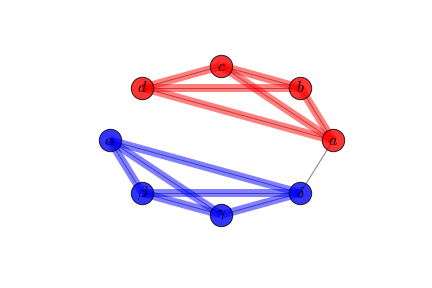
\includegraphics[width=\linewidth]{labels_and_colors_1.png}
  \caption{Instantiation 1 of SBM with $p=1.0$, $q=0.15$.}\label{fig:awesome_image1}
\endminipage\hfill
\minipage{0.32\textwidth}
  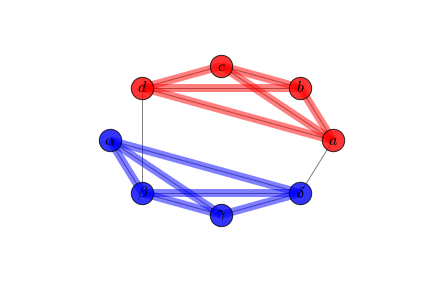
\includegraphics[width=\linewidth]{labels_and_colors_2.png}
  \caption{Instantiation 2 of SBM with $p=1.0$, $q=0.15$.}\label{fig:awesome_image2}
\endminipage\hfill
\minipage{0.32\textwidth}%
  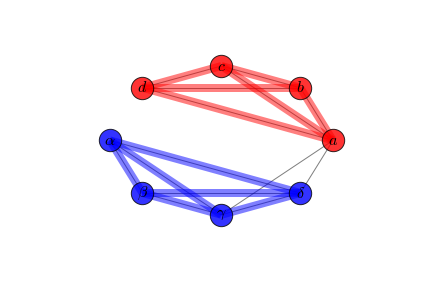
\includegraphics[width=\linewidth]{labels_and_colors_3.png}
  \caption{Instantiation 3 of SBM with $p=1.0$, $q=0.15$.}\label{fig:awesome_image3}
\endminipage
\end{figure}


So why is clustering on the SBM hard?  Clustering the above three graphs seem easy to do, but let's consider another example.  

\begin{figure}[h]
\begin{center}
  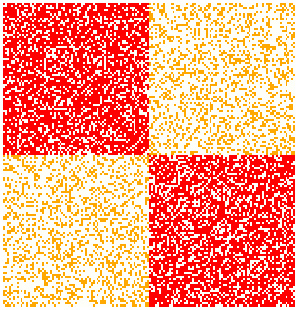
\includegraphics[scale=0.5]{SBM}
  \caption{Coloured and ordered adjacency matrix of SBM. Figure taken from \cite{SBM_adjacency_talk}}
  \label{fig:SBM_matrix_colour}
 \end{center}
\end{figure}

Figure \ref{fig:SBM_matrix_colour} is a coloured adjacency matrix representation of a SBM graph. Here we represent the adjacency matrix by colouring a square in figure \ref{fig:SBM_matrix_colour} if there is an edge, and leaving it white if there is no edge.  The red and yellow colouring differentiates the different community membership relationships (red for edges that are between two vertices of the same community, and yellow for edges between nodes that differ in their community membership). The number of nodes $n$ is much bigger in figure \ref{fig:SBM_matrix_colour} than in figure \ref{fig:awesome_image1}. Clearly $p$ and $q$ also don't seem too far apart.  Although the difference is still perceptible in the densities of the red and yellow regions, it is not a great difference.  In a real clustering problem we don't know the actual colouring, as in the case in figure \ref{fig:SMB_uncolored}.

\begin{figure}[h]
\begin{center}
  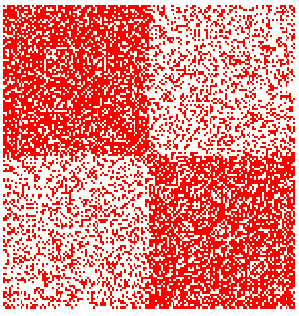
\includegraphics[scale=0.5]{SMB_uncolored}
  \caption{Ordered by uncoloured SBM adacency matrix.  Figure taken from \cite{SBM_adjacency_talk}}
  \label{fig:SMB_uncolored}
 \end{center}
\end{figure}

And most importantly, we don't actually know the order of the nodes as is the case in figure \ref{fig:SMB_unordered}. As in the previous two representations of the same graph, we ordered the nodes so that the nodes of one community proceed the other.  Of the $n\!$ permutations, there's only a few that makes that true, a diminishing small percentage of the total possible number of orderings of $n$ nodes.  

\begin{figure}[h]
\begin{center}
  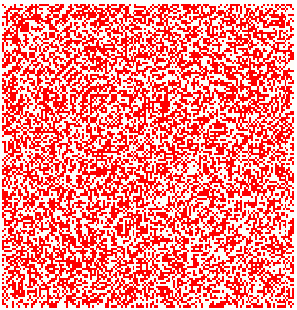
\includegraphics[scale=0.5]{SBM_unordered}
  \caption{Uncoloured and unordered adjacency matrix of SBM.  Figure taken from \cite{SBM_adjacency_talk}}
  \label{fig:SMB_unordered}
 \end{center}
\end{figure}

In \ref{fig:SMB_unordered} we don't have any hope of eyeballing all possible partitions of this graph into two communities.  

\section{Regimes of Clustering: Sparse to Dense}

One of the things figures \ref{fig:SBM_matrix_colour}, \ref{fig:SMB_uncolored}, and \ref{fig:SMB_unordered} help highlight is how much more difficult clustering can be if the difference between $p$ and $q$, the in-community probability of connecting and out-community probability of connecting (respectively), is small.  In fact, there is a rigorous quantification of this heuristic, as it drives a dichotomy in the quality of community recovery we can achieve. 
To talk about asymptotic behaviour of the SBM, let's confine our discussion to the the balanced SBM with two communities.  The definitions are easily extendable to SBM in general, however focusing on this balanced two community SBM makes clear what is being held constant and what is growing when we talk about asymptotic behaviour. 


\begin{definition}
We say a clustering of SBM(n, p, q) gives an \textit{Exact Recovery} if the probability of estimating the correct cluster assignments on SBM(n,p,q) goes to one as the number of nodes $n$ grows.  A clustering of the nodes $\{1, 2, ..., n\}$ is a partition of the nodes into communities.  We can encode that as a binary valued function $F : V \rightarrow \{0,1\}$ in the case of the two community SBM(n, p, q). So the exact recovery regime can be stated as $$\mathbb{P}( F_n = \bar{F_n}) \rightarrow_n 1$$  where $F_n$ corresponds to the correct clustering for SBM(n, p, q) and $\bar{F_n}$ is the predicted cluster assignments.   
\end{definition}

\begin{definition}
We say the clustering of SBM(n,p,q) gives \textit{detection} of the true communities if the predicted clusters correlate with the true communities.  Using the same $F_n$ (true community assignments) and $\bar{F_n}$ (predicted community assignments) as above, that means $$\exists \epsilon > 0 : \mathbb{P}(|F_n-\bar{F_n}| \geq 1/2+\epsilon) \rightarrow_n 1.$$ To adapt this definition to SBMs with $k$ communities, the $1/2$ inside the probability changes to $1/k$.  
\end{definition}

The detection regime is not just a weaker regime, it is actually impossible to obtain exact recovery for some families of $\{$SBM(n,p,q)$\}_n$.  Consider for instance when the SBM is not connected. In that case, the isolated vertices would have underdetermined community membership.  See figure \ref{fig:sparse} for a diagram of such an SBM. The results in \cite{MNS} prove what sparse regimes of the 2 community SBM allow for partial recovery.  


\begin{figure}[h]
\begin{center}
  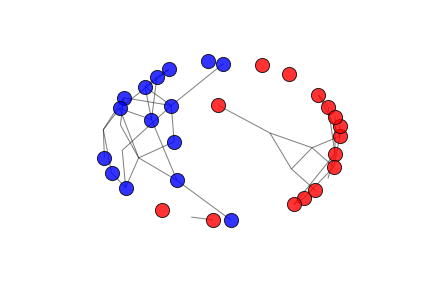
\includegraphics[scale=0.5]{SBM_balanced_large_sparse.png}
  \caption{Underdetermined labels due to isolated vertices.}
  \label{fig:sparse}
 \end{center}
\end{figure}

\subsection{Algorithmic Challenge}

In terms of the algorithmic challenge, the optimization problem is quite clear.  We are trying to find a graph partition that satisfies the minimum cut problem.  This problem is famously known to be $NP$-hard. In the balanced communities (communities of the same size) case, the problem is $NP$-complete.  For large $n$ graphs, we want to do better than just brute force go through all possible partitions.  Here relaxing the problem has presented many opportunities to apply spectral algorithms, semi-definite programming and belief propagation methods.  Since spectral methods have been shown to achieve the information theoretic threshold mentioned in the previous section, and because it provides the inspiration for our Graph Neural Network model, we will give an exposition of spectral clustering algorithms here.  

\section{Spectral Clustering for the SBM}

Spectral clustering is based on studying the spectrum of the graph Laplacian.  


Let $G= (V, E)$ be a graph, possibly weighed graph where $\{w_{ij}\}$ are the weights.  The degree of vertex $v_i$ is given by 
$$ d_i := \sum_{j=1}^n w_{ij}.$$

The degree matrix $D$ then is the diagonal matrix with entries $d_1, ..., d_n$ along its diagonal. Let $W$ be the adjacency matrix of $G$.  

\begin{definition}The \textit{unnormalized graph Laplacian} is defined as

$L : = D-W.$ 
\end{definition}
\begin{definition}The \textit{symmetric graph Laplacian} is defined as

$L_{sym} : = I - D^{-1/2}WD^{-1/2} = D^{-1/2}LD^{-1/2}.$ 
\end{definition}
\begin{definition}The \textit{random walk Laplacian} is defined as

$L_{rw} : = I - D^{-1}W = D^{-1}L.$ 
\end{definition}

The graph Laplacians above enjoy some nice properties.  In particular: 

\begin{prop}{\cite{tutorial_SC}}
\begin{itemize}
    \item For every $v \in \mathbb{R}^n$ we have
    $$v L v^T = \frac{1}{2}\sum_{i,j =1}^nw_{ij}(v_i-v_j)^2.$$
    \item $L$ is symmetric and positive semi-definite.
    \item The smallest eigenvalue of $L$ is 0, the corresponding eigenvector is the constant one vector \textbf{1}. $0$ is also an eigenvalue of of $L_{rw}$ and $L_{sym}$, corresponding to the constant one vector \textbf{1} and $D^{-1/2}$as eigenvectors respectively. 
    \item $L$ has $n$ non-negative, real-valued eigenvalues $0 = \lambda_1 \leq \lambda_2 \leq ...\leq \lambda_n$. 
\end{itemize}
\end{prop}

 Spectral clustering algorithms generally use some version of graph Laplacians, either one of the three classical ones above, or some matrix that is a perturbation of a Laplacian.  We will discuss one such perturbation when we define the Bethe Hessian matrix in the next chapter.  As for the steps of a generic spectral clustering algorithm, it follows roughly the following algorithm.  

\begin{algorithm}[H]
 \textbf{Input: } A graph adjacency matrix $W$ corresponding to graph $G = (V, E)$. Let $k$ be the number of clusters desired.
 
 \begin{enumerate}
    \item Create $L$, $L_{sym}$, $L_{rw}$ from $W$.  Let us call the matrix we are finding the spectrum of $Q$. 
    \item Take eigendecomposition of $Q$.  
    \item Take the $k$ dimensional eigenspace associated with biggest or smallest eigenvalues of Q. Choose the eigenspace corresponding to the biggest eigenvalues if $Q = L$, and the eigenspace corresponding to the smallest eigenvalues if $Q= L_{sym}$ or $Q = L_{rw}$.  
    \item Project the vertices $v \in V$ onto this $k$ dimensional subspace.
    \item Perform the k-means algorithm on the projected vertices. 
 \end{enumerate}
 
 \textbf{Output:} A clustering of the vertices $v$ into $k$ clusters.  This can be encoded as a function $F: V \rightarrow \{1,2,...,k\}$.
 
 \caption{General Spectral Clustering Algorithm}
\end{algorithm}


Choosing what matrix to use for $Q$ (defined in the algorithm above) is somewhat of an art in clustering problems, especially when it comes to applying it to real data.  In the case of generative models, we have a better understanding of what the cuts should look like.  Are we minimizing cuts while normalizing by volume?  Is our graph extremely sparse that the extreme eigenvalues exhibit large fluctuations?  In short, there are many versions of spectral algorithms that differ on what matrix the spectral algorithm is applied to.  A bulk of them is based on the Laplacian, some on other matrices we can derive from the adjacency matrix of a network. 

One way of seeing how spectral clustering works is to regard the spectral decomposition as a particularly useful embedding of $v \in \mathbb{R}^n$ (as represented by the adjacency matrix) to $\bar{v} \in R^k$ (where $k$ is how many clusters we want to extract).  The eigenbasis is informative because it provides us the most extreme directions that highlights where connections are most sparse (the eigenproblem is in fact a relaxation of min cut).  For instance, consider an instantiation of SBM($n =40, (p = 0.5, q = 0.05)$).  Here $k = 2$.  In figure \ref{fig:randomproj} and figure \ref{fig:spectralproj} we compare a random projection of our vertex set to $\mathbb{R}^2$ with a projection using the spectral basis.  

\begin{figure}[h]
\minipage{0.4\textwidth}
  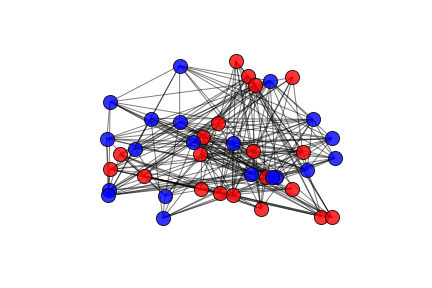
\includegraphics[scale=0.6]{SBM_balanced_large_dense_rand.png}
  \caption{Random Embedding}
  \label{fig:randomproj}
\endminipage\hfill
\minipage{0.4\textwidth}
  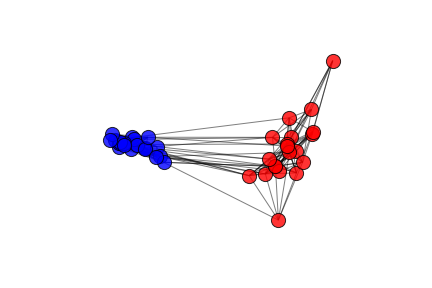
\includegraphics[scale=0.6]{SBM_balanced_large_dense_spectral.png}
  \caption{Spectral Embedding}
  \label{fig:spectralproj}
\endminipage\hfill
\end{figure}


\section{Thresholds for Detectability and Exact Recovery}
In this section we discuss what is the relationship between parameters of the SBM and the performance of clustering algorithms.  To characterize this relationship, we need to use the constant degree parametrization of the SBM so that we can talk about sparse and dense graphs.  In particular, in the two balanced community SBM$(n,p, q)$ we can reparametrize with $a :=  p \cdot n$ and $b := q \cdot n$.  Where $a, b$ are the average within-community and out-of-community average degrees respectively.  The regimes where exact recovery and detection can be made are the following (the definitions of exact recovery and detection were given in section 8.1). 

\begin{definition}The \textit{exact recovery information threshold} is the point in which we cannot  recover the correct community labels with probability one in the limit.  Given $p=\frac{alog(n)}{n}, q = \frac{b log(n)}{n}$, we can only achieve exact recovery if and only if $\frac{a+b}{2} \geq 1 + \sqrt{ab}$ as was shown in \cite{MNS} and \cite{ABH}. 
\end{definition}

 In \cite{MNS}, Mossel, Neeman, and Sly provide a polynomial time algorithm that is capable of recovering the parameters in the exact recovery threshold (the threshold which they prove below which no algorithm can recover the communities).  The proof has three stages. First classical spectral clustering is to compute an initial guess. A replica stage is then used to reduce error by holding out subsets and repeating spectral clustering on remaining graph.  And finally, on a small number of uncertain labels, majority rule to refine their assignments. Abbe, Bandeira and Hall showed in \cite{ABH} that they can provide an algorithm using semi definite programming to achieve the state of the art in the same sparse regime as above. 

\begin{definition}
The \textit{detection information theoretic threshold} applies to the SBM with paramters $p = \frac{a}{n}, q = \frac{b}{n}$. That is, when there is a constant degree sequence of SBM graphs as $n\rightarrow \infty$. It was shown in \cite{MNS_sparse}, \cite{Massouli} and \cite{AFL} that detection is possible if and only if $(a-b)^2 > 2(a+b)$.
\end{definition}

Mossel, Neeman and Sly showed in \cite{MNS_sparse} that they can do partial recovery with spectral clustering with initial guess, then finish the algorithm with belief propagation to refine the guess.  Massoulie showed in \cite{Massouli} that spectral clustering can be applied successfully in this regime using the non-backtracking matrix, a matrix that counts the number of non backtracking paths from each vertex of a given length.   Saade, Krzakala and Zdeborová showed in \cite{AFL} that a type of deformed Laplacian via a 1-dim parameter that shares eigenvalues with non-backtracking matrix for spectral decomposition can be used successfully in this regime.  This deformation Laplacian is called the Bethe Hessian.    

   
Note first that these results are all very recent. They are also not trivial.  The proofs require tools form random matrix theory, the theory of branching processes and semi definite programming, to name a few, so a fairly deep level of machinery and theory was required. Also notice that in each regime there is a spectral approach that can successfully achieve recovery/detection down to the information theoretic threshold.  The only catch is the what type of matrix to apply the spectral method to.  Thus the takeaway is that there is no one size fits all model. Clustering, even in the two community case of the SBM requires a lot of expertise to refine the right matrices whose spectrum will amplify the signals required to achieve detection/recovery up to the information theoretic threshold. 

Given all this, the present work's contribution is the following.  We will design a neural network architecture that is expressive enough to approximate these spectral algorithms.  Then we will show that the GNN can achieve detection down to the information theoretic threshold, thus showing the GNN is competitive with the state of the art algorithms while requiring less computational steps. % And finally, perhaps most importantly, show that these models can be applied successfully to real data, and provide a computationally efficient approach.
The nice thing about bringing neural networks to bear on the problem is to let gradient descent replace the``ingenuity" aspect of clustering.  We no longer need to meticulously choose the right matrices to apply spectral clustering to.  Gradient descent will learn the correct parameters, in a data driven way. 
